%(subject) (theme) (title)
\documentclass[11ptm]{jsarticle}

\usepackage{etoolbox}

\usepackage{array}

\usepackage{enumitem}

\usepackage{amsmath, newtxmath}

\usepackage[dvipdfmx]{graphicx}
%\usepackage[draft, dvipdfmx]{graphicx}

\usepackage[hang, small, bf]{caption}
\usepackage[subrefformat=parens]{subcaption}
\captionsetup{compatibility=false}

\usepackage{listings, jlisting}

\lstset{
  basicstyle={\ttfamily\small},
  frame=tbrl,
  breaklines=true,
%  language=C,
  lineskip=-0.5ex,
  tabsize=2
}

\usepackage{tabularx}% 表(改変履歴)のため

\usepackage{hyperref}% ハイパーリンク付き参照
\usepackage{pxjahyper}% ハイパーリンク内の日本語の文字化け防止

\usepackage[margin=20mm]{geometry}% 余白調整用
% geometry settings
\renewcommand{\baselinestretch}{0.78}% 行間を少し狭める
% geometry settings

\usepackage{fancybox}% fbox以外のboxコマンドを導入

\usepackage{fancyhdr}% ヘッダー・フッター装飾
% fancyhdr settings
\pagestyle{fancy}
\lhead{{\small\bf 管理者向けマニュアル}}
\rhead{{\small\bf \leftmark}}
% fansyhdr settings end.

\makeatletter
\AtBeginDocument{
\let\c@figure\c@lstlisting
\let\thefigure\thelstlisting
\let\ftype@lstlisting\ftype@figure
}
\makeatother

\title{{\Huge POaM資産管理システム(仮称)\\操作マニュアル\\}管理者ユーザ向け\\\Huge{第2版}}
\author{24 高橋祥吾\\26 田桑大輔\\29 田中稀尋\\30 谷川僚}
\date{}

%見出しの表示形式を再設定
\renewcommand{\thepart}{\arabic{part}}
\renewcommand{\thesection}{\ \arabic{section}章}
\renewcommand{\thesubsection}{\ \arabic{section}.\arabic{subsection}}

%%%%%%%%%%%%%%%%%%%
%%%%%%%%%%%%%%%%%%%
\begin{document}

%%%%%%%%%%
%タイトル
\setcounter{page}{0}

\maketitle
\thispagestyle{empty}

\clearpage

%%%%%%%%%%
%目次
\setcounter{page}{0}
\thispagestyle{empty}

\tableofcontents
\clearpage


% %%%%%%%%%%
% %\clearpage
% \section{マニュアルとは}
% \label{sec:マニュアルとは}
% マニュアルには種類がある。
% \begin{itemize}
%   \item 操作マニュアル
%   \item 業務マニュアル
%   \item 障害対応マヌカハニー
%   \item システムマニュアル
% \end{itemize}\par
% それぞれについて少し解説する。\par
% 操作マニュアルとは、システムの使い方、操作方法を記述するマニュアル。システムの起動や終了の仕方をはじめ、システムが備えるすべての機能の使い方、その機能を使う際の操作方法を詳細に記述。\par
% 業務マニュアルとは、システムを使った業務の進め方を記述するマニュアル。ひとつひとつの業務の流れ・手順を記述するとともに、流れ・手順のどの時点でシステムのどの機能を使うのかがわかるように記述する。機能の使い方や操作方法を記述する必要はない(操作マニュアルに任せる)。\par
% 障害対応マニュアルとは、システムに障害が生じたときの対応処理の方法を記述したもの。ただし、エンドユーザが自力で対応・解決できる範囲の障害だけに限る。要はQ$\&$A。\par
% システムマニュアルとは、システムの仕組みや構造・全体的な構成などを基本からわかりやすく説明したもの。エンドユーザ向けであり、システム管理者やエンジニア向けのマニュアルのような詳細かつ専門的なものではなく、入門レベルの概要的なものになる。\\\par
% 我々が制作するのは授業的には操作マニュアルのみで十分だが、その他のマニュアルを制作してもソフトウェア工学の点数として評価される。また、障害対応マニュアルの一部を掲載すると丁寧。


% %%%%%%%%%%
% %\clearpage
% \section{わかりやすい操作マニュアル制作のポイント}
% \label{sec:わかりやすい操作マニュアル制作のポイント}
% \url{https://www.science.co.jp/document_blog/26059/}

% %%%%%
% %\clearpage
% \subsection{そもそも操作マニュアルとは}
% \label{sec:そもそも操作マニュアルとは}
% 操作マニュアルとは文字通り、システムの操作方法を確認するためのドキュメント。マニュアルという立場上、操作マニュアルの多くは初心者や何も知らない顧客向けに作成される。よって、操作マニュアルの作成者は以下の点を意識する必要がある。
% \begin{itemize}
%   \item 初心者にも操作が理解しやすく記載されており、読後正しく操作ができる
%   \item システムや機械を操作したあと、正しい操作だったかどうか、正解がわかる
%   \item 困ったときに、すぐに該当のページに辿り着ける
% \end{itemize}\par
% 世の中には、とりあえず操作手順を全部載せましたというマニュアルが存在している。分厚いだけのマニュアルは読み手の意欲を下げるので、ほとんど読まれることがない。また、直感的に操作できるシステムでは、作成しても操作マニュアルが読まれないケースがある。このような操作マニュアル未読のケースは、操作ミスや意図しない事故を発生させる可能性があり、大変危険である。\par
% 操作マニュアルの作成者は、先ほど挙げた3点を常に意識し、読了してもらえる操作マニュアルを完成しよう。

% %%%%%
% %\clearpage
% \subsection{制作のポイント5つ}
% \label{sec:制作のポイント5つ}
% \begin{enumerate}
%   \item 操作説明は網羅的に記載する
%   \item 疑問点や注意事項は記載しておく
%   \item 視覚的要素を用いる
%   \item 操作の目的を記載する
%   \item 操作の結果を記載する
% \end{enumerate}
% 「Google検索からYahoo!のHPを開く」というケースで説明。

% %%%%%
% %\clearpage
% \subsubsection{操作説明は網羅的に記載する}
% \label{sec:操作説明は網羅的に記載する}
% 操作方法は細かいと良い。ただし冗長なものはわかりにくくなる。\par
% 操作内容の他にも、作業順、作業タイミング、操作者、条件などを記載するとよりわかりやすくなる。\par
% \begin{lstlisting}
% PC操作者 : Googleの検索バーに「yahoo」と打ち込み、Enterキー押下
% 検索結果が表示される
% PC操作者 : 検索結果の一番上にある「Yahoo!JAPAN」をクリック
% Yahoo!のHPを表示
% \end{lstlisting}

% %%%%%
% %\clearpage
% \subsubsection{疑問点や注意事項は記載しておく}
% \label{sec:疑問点や注意事項は記載しておく}
% 操作にある程度慣れてくると疑問が湧くことがある。今回のケースで言えば、「Googleの検索履歴にYahoo!があるが、選択してもよいのか」など。このような疑問に対して、「入力履歴を選択しても問題ありません」などと記載しておくと、よりユーザビリティの高いマニュアルとなる。\par
% また、注意事項や禁止操作も同時に記載すると良い。とはいえあらゆる疑問について記載していてはキリがないので、Q$\&$Aへ誘導するなどして、可読性とのバランスは取ったほうが良い。

% %%%%%
% %\clearpage
% \subsubsection{視覚的要素を用いる}
% \label{sec:視覚的要素を用いる}
% 文字だけでなく図や画像などを併せて操作マニュアルを記述しよう。

% %%%%%
% %\clearpage
% \subsubsection{操作の目的を記載する}
% \label{sec:操作の目的を記載する}
% 操作の目的を記載することで全体像の把握につながる。全体像の把握は作業効率の向上や作業重要性の理解につながる。\par
% また、目次が目的ごとに並んでいれば、検索性が格段に上がる。自分のやりたい操作とページが瞬時に紐づくことで、作業が滞りなく進む。

% %%%%%
% %\clearpage
% \subsubsection{操作の結果を記載する}
% \label{sec:操作の結果を記載する}
% 今回のケースでいえば、以下のようなところ。
% \begin{lstlisting}
%   PC操作者 : Googleの検索バーに「yahoo」と打ち込み、Enterキー押下
%   検索結果が表示される
% \end{lstlisting}

%%%%%%%%%%%%%%%%%%%%
%\clearpage
\part{前文}
\hrulefill


%%%%%%%%%%
%\clearpage
\section{はじめに}
\label{sec:はじめに}
POaM資産管理システム(以下、本システム)は、本校の資産を円滑かつ簡潔に管理するための、ブラウザ上で動作するオンラインWebアプリケーションです。\par
このPOaM資産管理システム操作マニュアル(以下、本マニュアル)は\ref{sec:動作環境}に則った環境を前提としています。システムを利用するためのURLにアクセスできない場合はネットワーク接続環境を確認してください。\par
また、本マニュアルは管理者権限を持ったユーザ向けです。


%%%%%%%%%%
%\clearpage
\section{動作環境}
\label{sec:動作環境}
IE9+のブラウザ


%%%%%%%%%%%%%%%%%%%%
\clearpage
\part{操作説明}
\hrulefill


%%%%%%%%%%
%\clearpage
\section{起動・終了}
\label{sec:起動・終了}

%%%%%
%\clearpage
\subsection{システムの起動}
\label{sec:システムの起動}
ブラウザを開き、URLに接続します。接続に成功すると、図\ref{fig:ログイン画面}が表示されます。ログインについては\ref{sec:ログイン}を参照してください。

%%%%%
%\clearpage
\subsection{システムの終了}
\label{sec:システムの終了}
ブラウザのタブを閉じることでシステムを終了できます。\par
登録などの資産に関する作業をしているとき、\ovalbox{完了}ボタンを押す前にシステムを終了した場合、作業内容は保存されません。


%%%%%%%%%%
%\clearpage
\section{ログイン}
\label{sec:ログイン}
登録されたメールアドレスとパスワードをフォームに入力し、\ovalbox{ログイン}ボタンを押すことでログインできます。\par
ログインするとホーム画面(図\ref{fig:ホーム画面})が表示されます。\par
パスワードの入力フォームの横にある\ovalbox{非表示中}ボタンを押すと、入力中のパスワードの伏字を外すことができます。
\begin{figure}[h]
  \centering
  \fbox{
    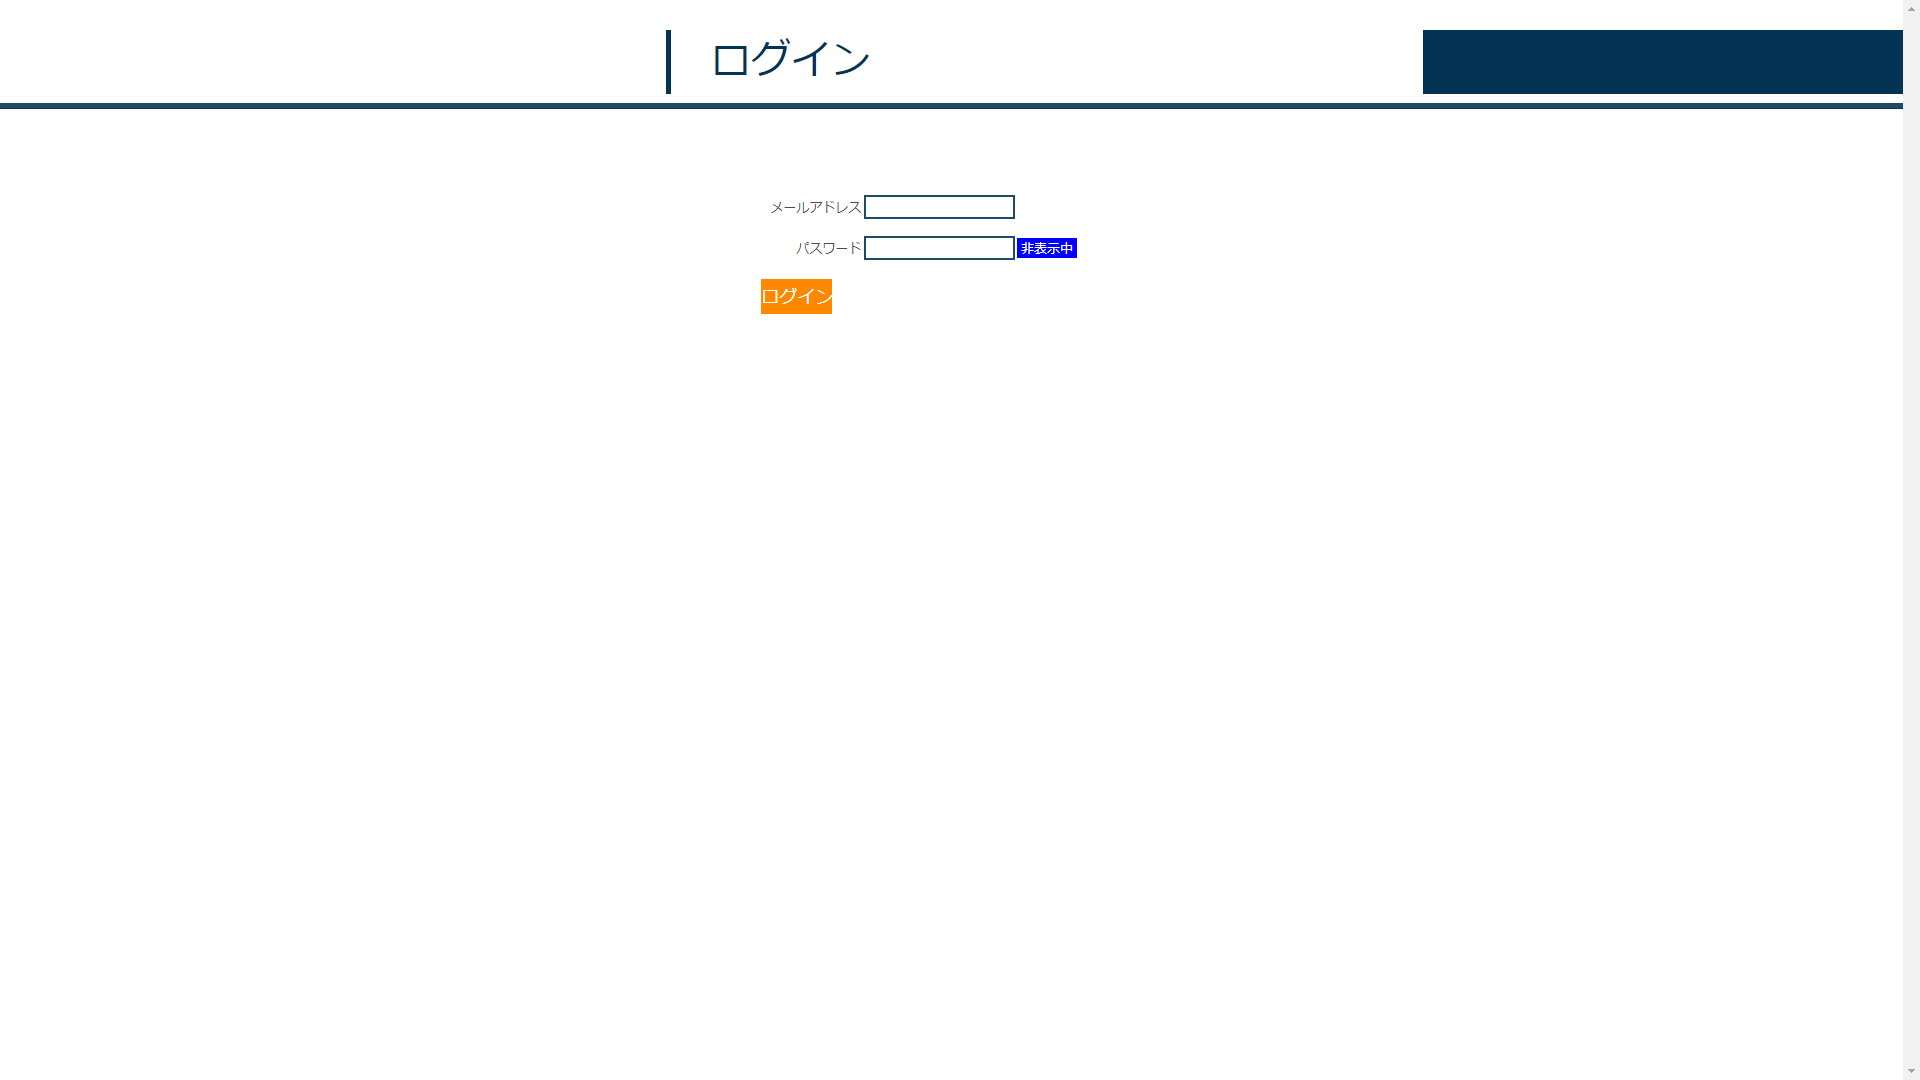
\includegraphics[keepaspectratio, width=0.8\linewidth]{source/login.png}
  }
  \caption{\label{fig:ログイン画面}ログイン画面}
\end{figure}


%%%%%%%%%%
%\clearpage
\section{ホーム画面}
\label{sec:ホーム画面}
ホーム画面からは、本システムの多くの機能にアクセスできます。アクセスできる機能は以下の通りです。
\begin{itemize}
  \item 資産の登録 (\!\ref{sec:資産の登録})
  \item ユーザ管理 (\!\ref{sec:ユーザの管理})
  \item 資産情報の検索 (\!\ref{sec:資産の検索})
\end{itemize}\par
\begin{figure}[h]
  \centering
  \fbox{
    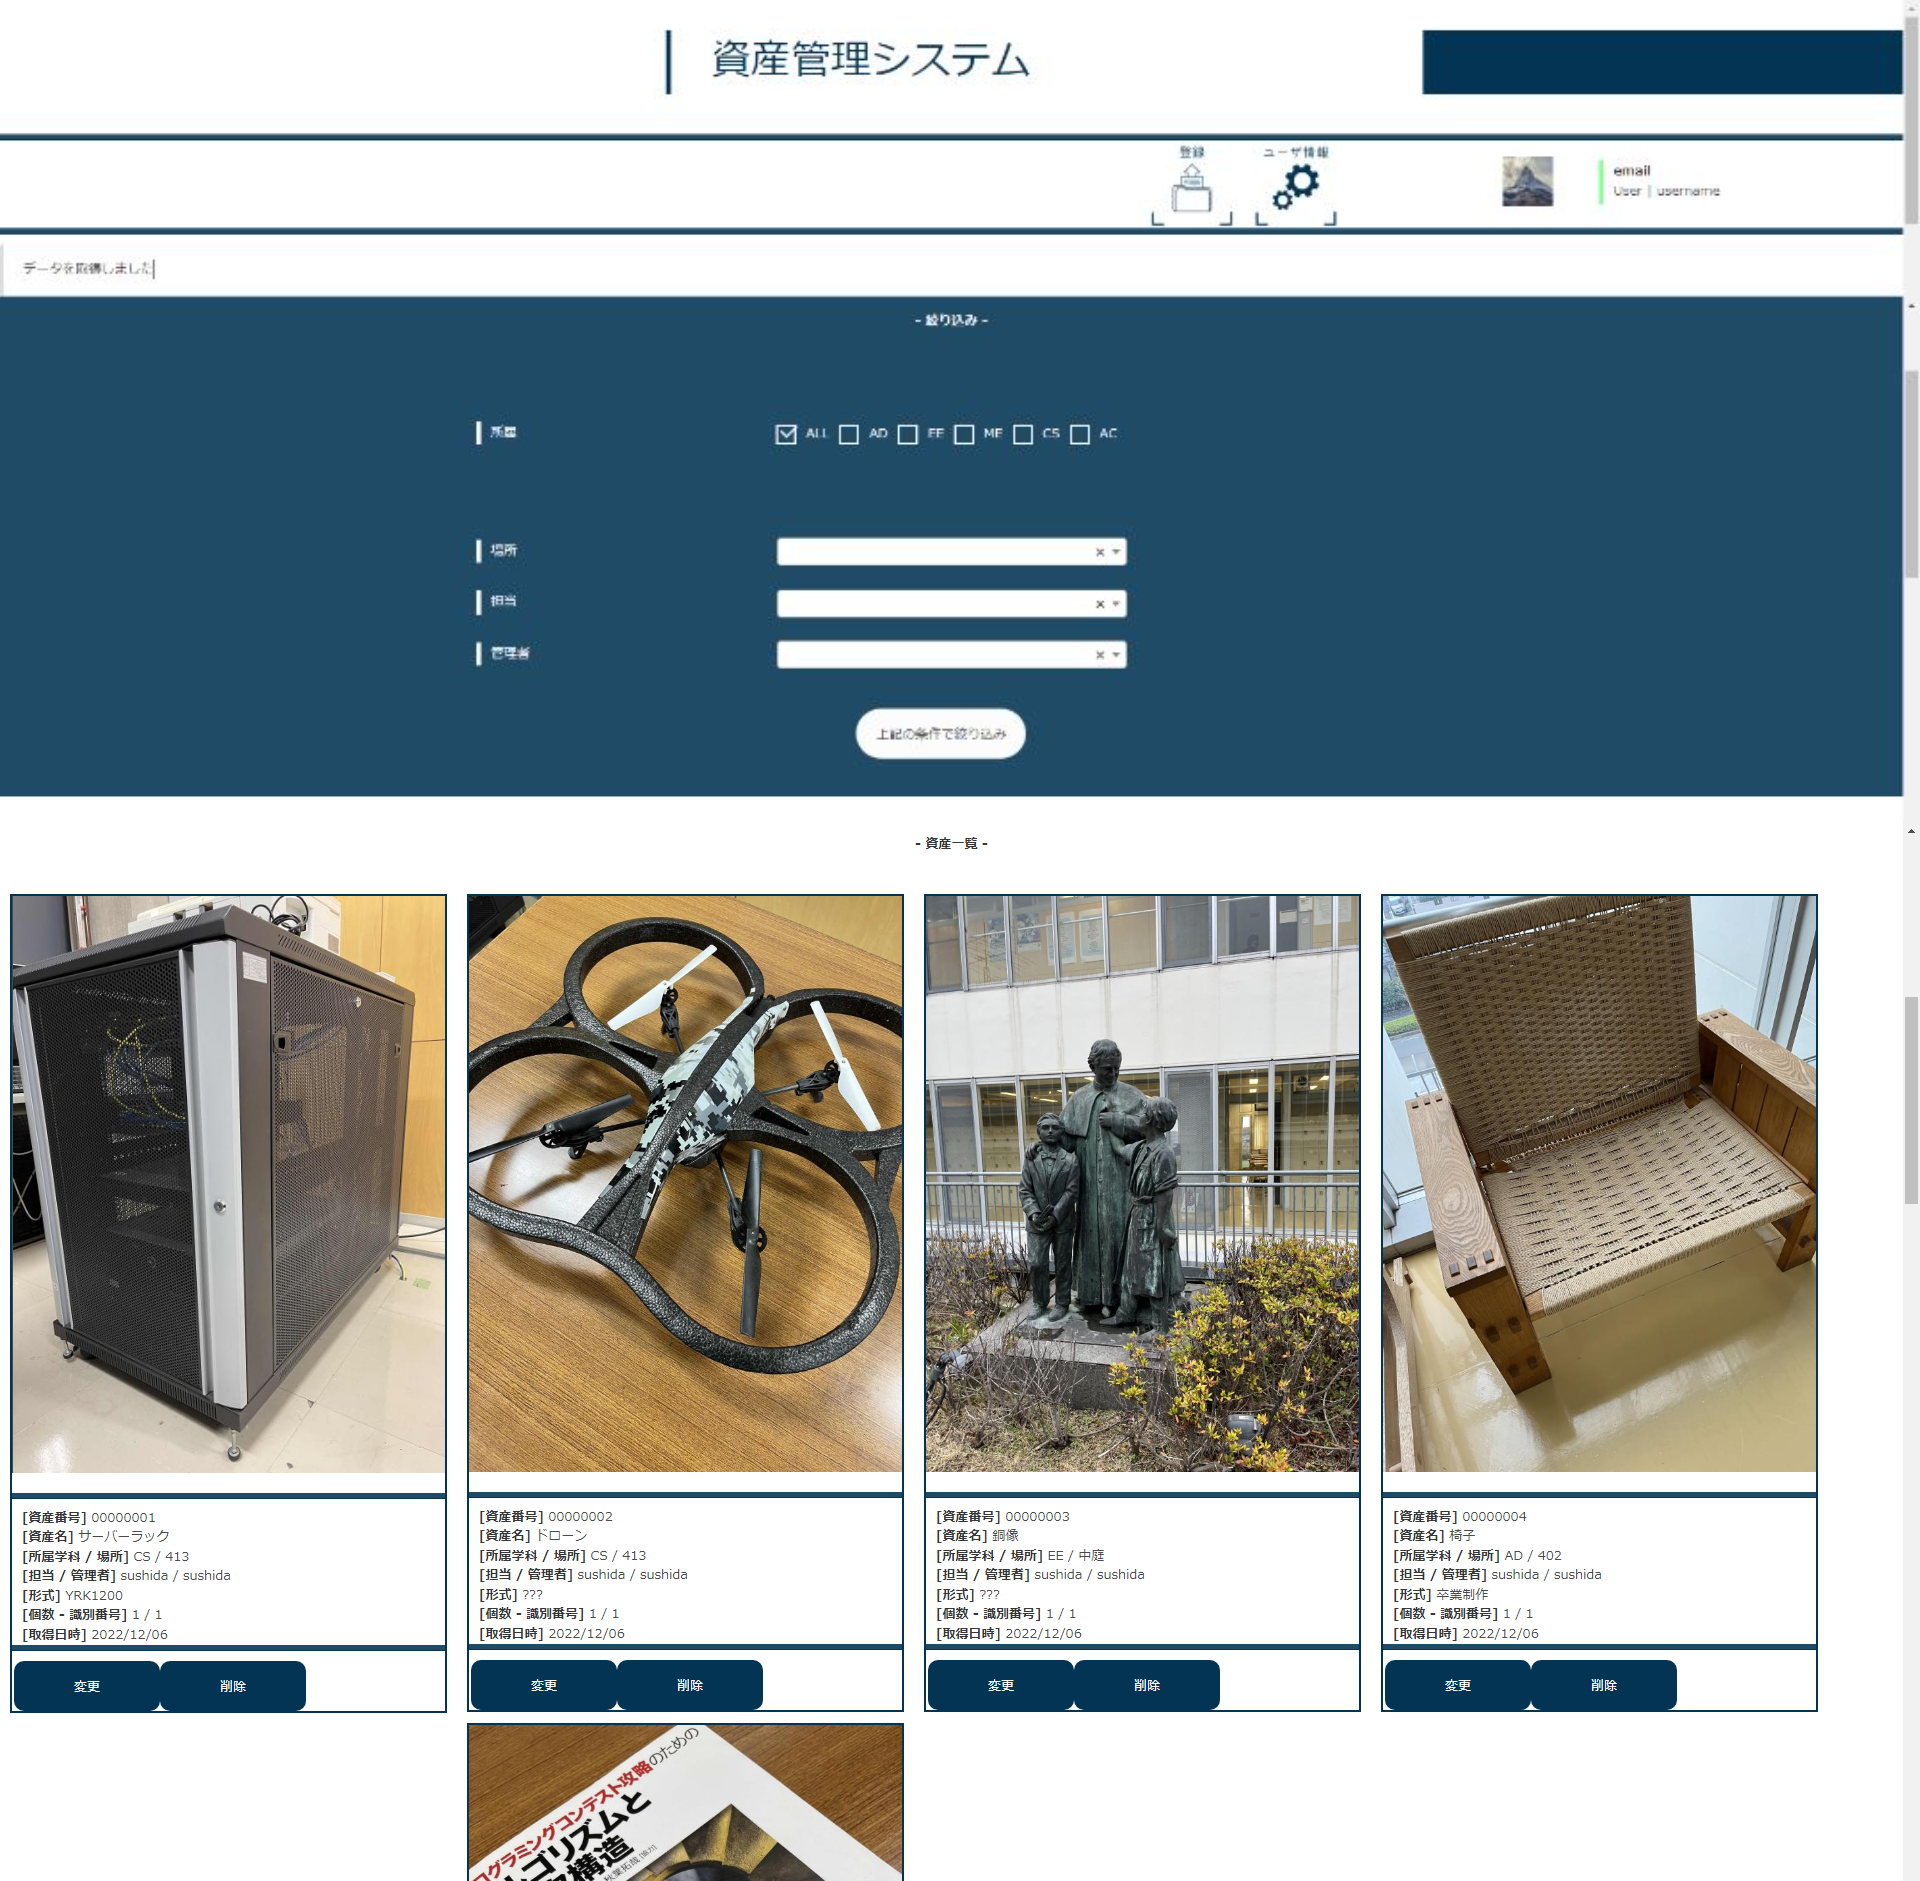
\includegraphics[keepaspectratio, width=0.8\linewidth]{source/home.png}
  }
  \caption{\label{fig:ホーム画面}ホーム画面}
\end{figure}


%%%%%%%%%%
\clearpage
\section{資産の登録}
\label{sec:資産の登録}
資産番号、所属、資産名、場所、担当者、管理者、形式、個数、取得年月日、画像のURLを入力できるようになっています(図\ref{fig:登録画面})。\ovalbox{入力内容を確認}ボタンを押すと確認画面(図\ref{fig:登録画面の確認表示})が表示され、\ovalbox{登録}ボタンを押すと登録できます。\par
%各項目について入力形式とか詳しく言うかどうか
%Core2Duoは各項目ごとにsubsectionをたてることで「登録手順」としていた 我々は画像で対応したい
%確認画面が表示されるところまで記載
%画像内の説明文をより詳しくするイメージで文章を記述する
\begin{figure}[h]
  \centering
  \fbox{
    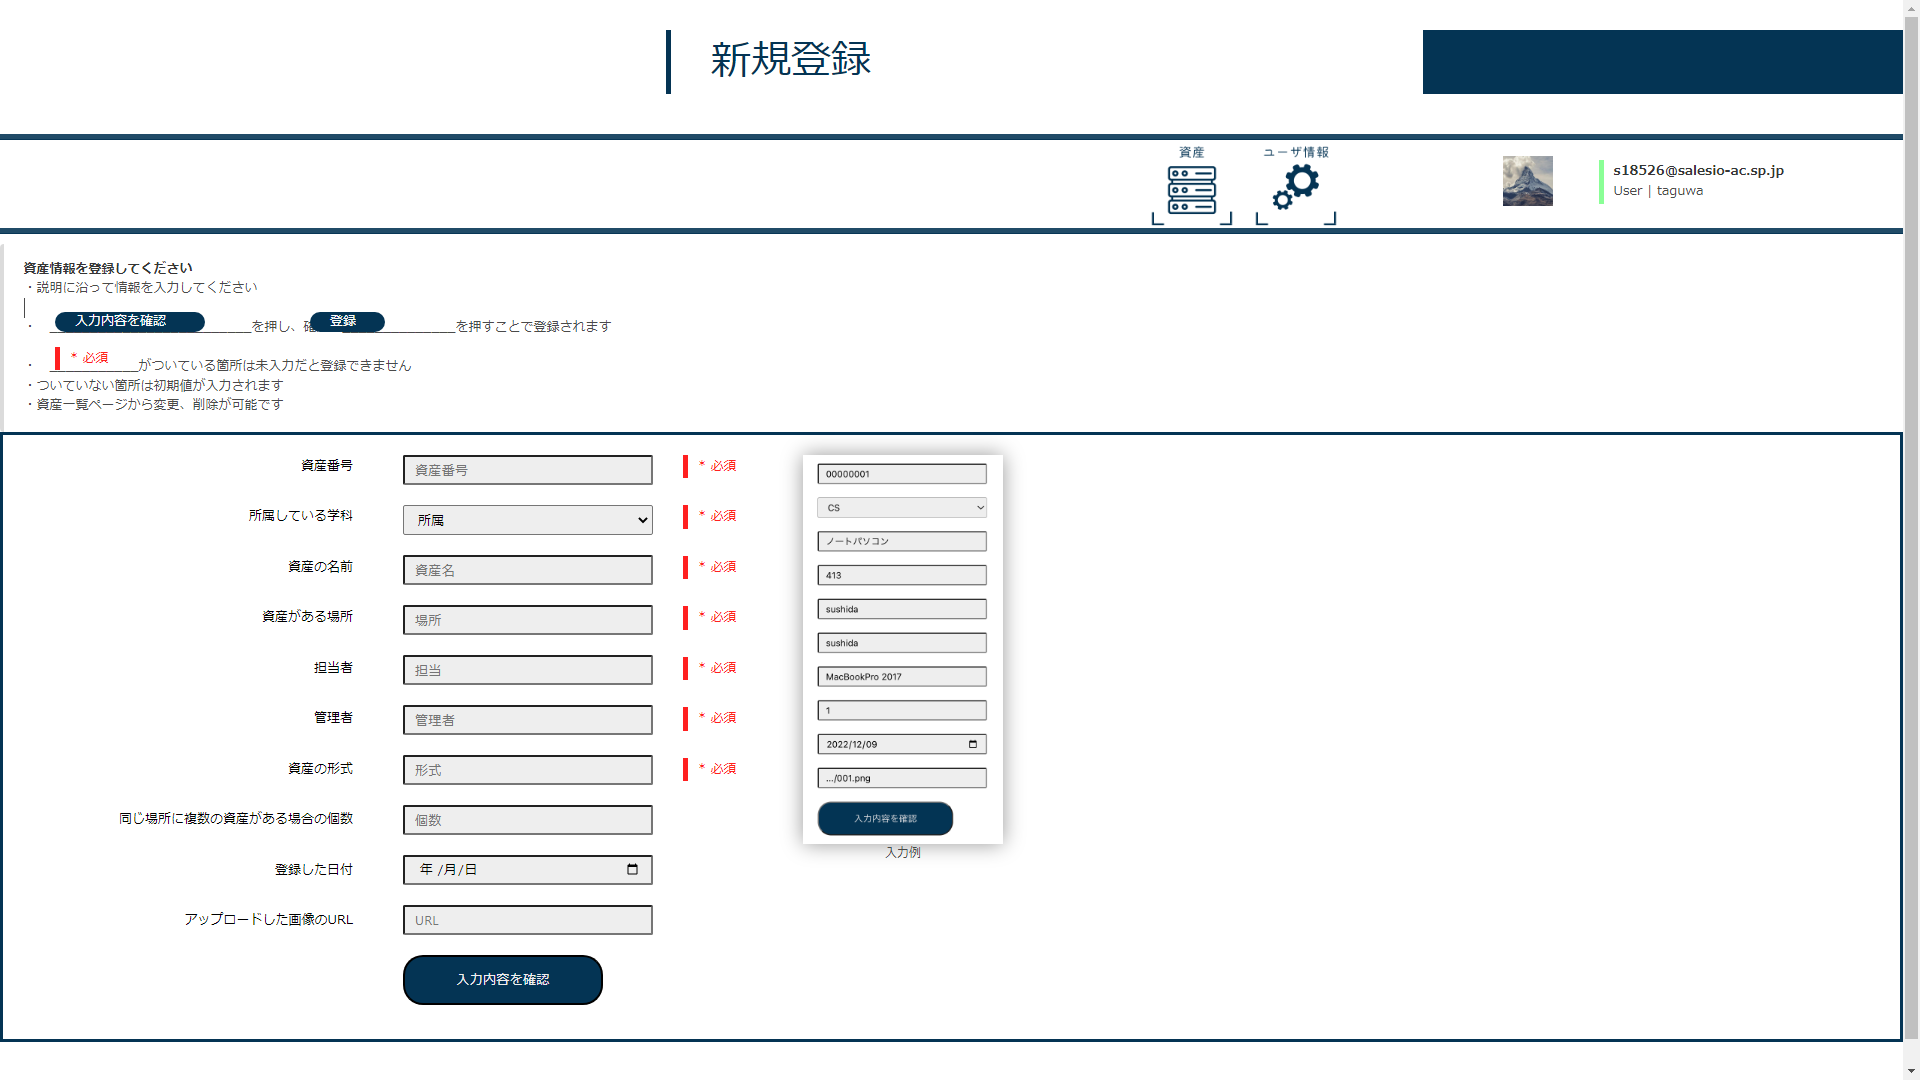
\includegraphics[keepaspectratio, width=0.8\linewidth]{source/submit.png}
  }
  \caption{\label{fig:登録画面}登録画面}
\end{figure}
\begin{figure}[h]
  \centering
  \fbox{
    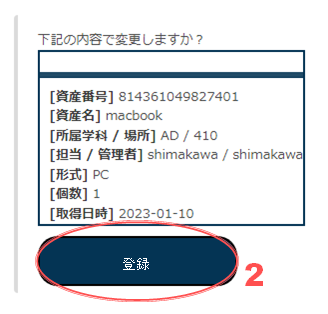
\includegraphics[keepaspectratio, width=0.8\linewidth]{source/submit_verification.png}
  }
  \caption{\label{fig:登録画面の確認表示}登録画面の確認表示}
\end{figure}


%%%%%%%%%%
\clearpage
\section{資産の検索}
\label{sec:資産の検索}
ホーム画面\ref{fig:ホーム画面}の下部で資産の検索を行えます。\par
検索は項目別に絞り込んで行えます。項目は所属、場所、担当、管理者となっており、これらを選択または入力して\ovalbox{上記の条件で絞り込み}ボタンを押すことで検索結果が変化します。
%検索画面のスクショが必要
\begin{figure}[h]
  \centering
  \fbox{
    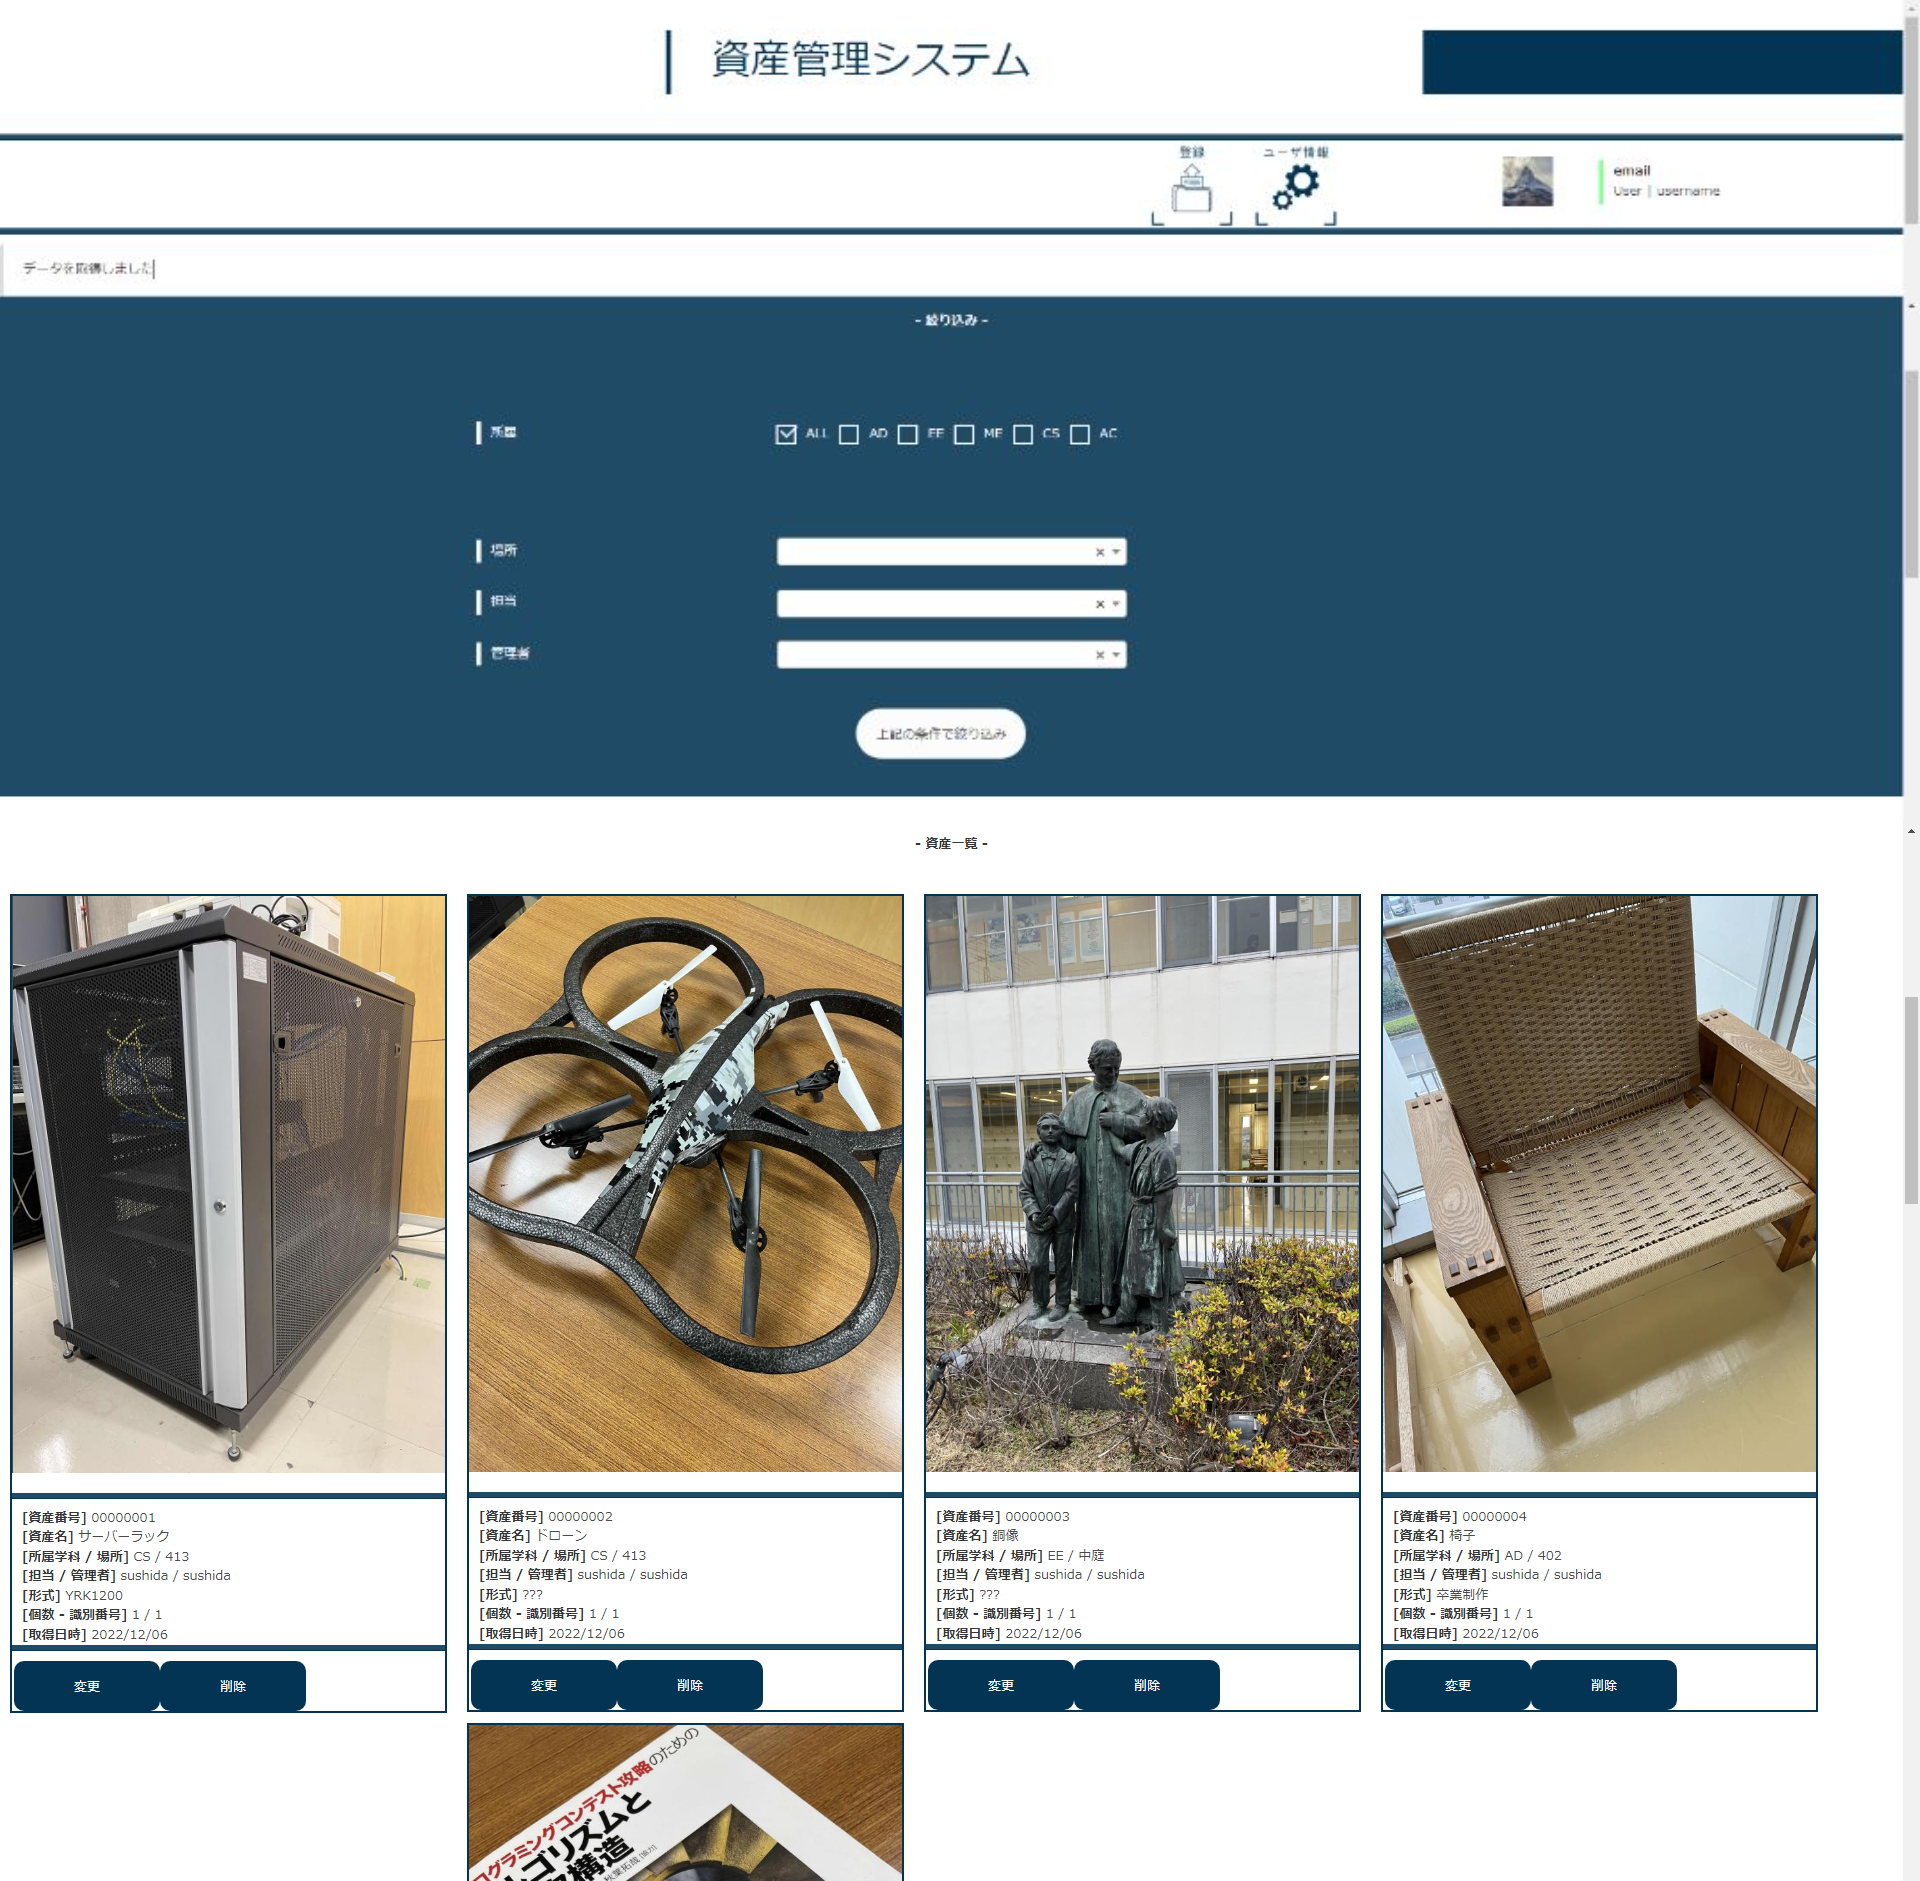
\includegraphics[keepaspectratio, width=0.8\linewidth]{source/home.png}
  }
  \caption{\label{fig:検索}検索}
\end{figure}


%%%%%%%%%%
\clearpage
\section{資産の編集}
\label{sec:資産の編集}
資産番号、所属、資産名、場所、担当者、管理者、形式、個数、取得年月日、画像のURLを入力できるようになっています(図\ref{fig:変更画面})。\ovalbox{入力内容を確認}ボタンを押すと確認画面(図\ref{fig:変更画面の確認表示})が表示され、\ovalbox{変更}ボタンを押すと登録できます。\par
%・登録と同じようにすればいいと思う\par
%・確認画面が表示されるところまで記載\par
%・画像内の説明文をより詳しくするイメージで
\begin{figure}[h]
  \centering
  \fbox{
    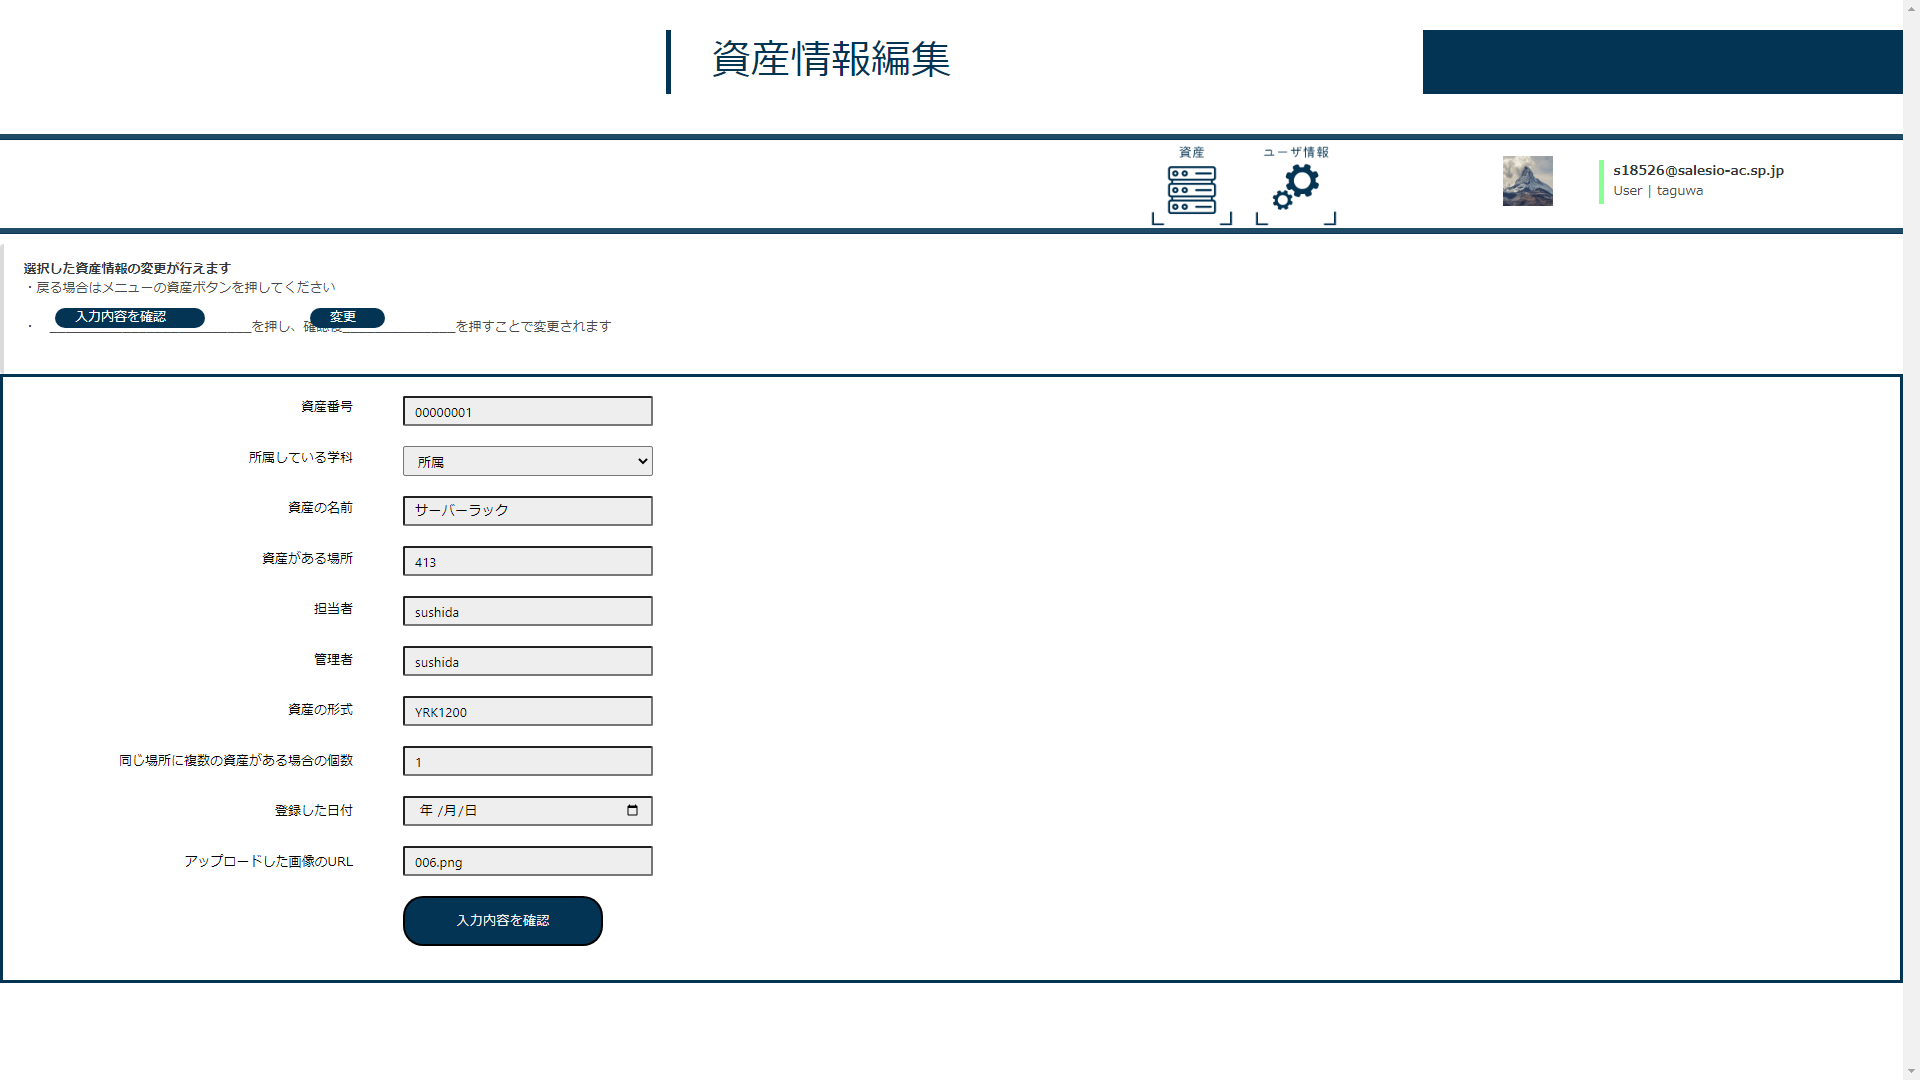
\includegraphics[keepaspectratio, width=0.8\linewidth]{source/change.png}
  }
  \caption{\label{fig:変更画面}変更画面}
\end{figure}
\begin{figure}[h]
  \centering
  \fbox{
    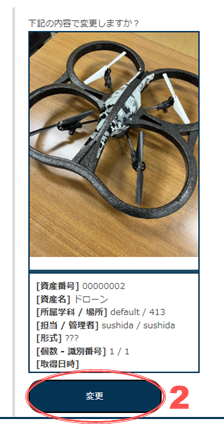
\includegraphics[keepaspectratio, width=0.8\linewidth]{source/change_verification.png}
  }
  \caption{\label{fig:変更画面の確認表示}変更画面の確認表示}
\end{figure}


%%%%%%%%%%
%\clearpage
\section{資産の削除}
\label{sec:資産の削除}
%・変更の画面からできることを考慮しないといけない絶対に


% %%%%%%%%%%
% %\clearpage
% \section{プロフィールの編集}
% \label{sec:プロフィールの編集}
% ログインしているユーザ(アカウント)のプロフィールを編集できます。編集できる項目はログインに利用するパスワードのみです。
% %・ユーザ情報編集
% \begin{figure}[h]
%   \centering
%   \fbox{
%     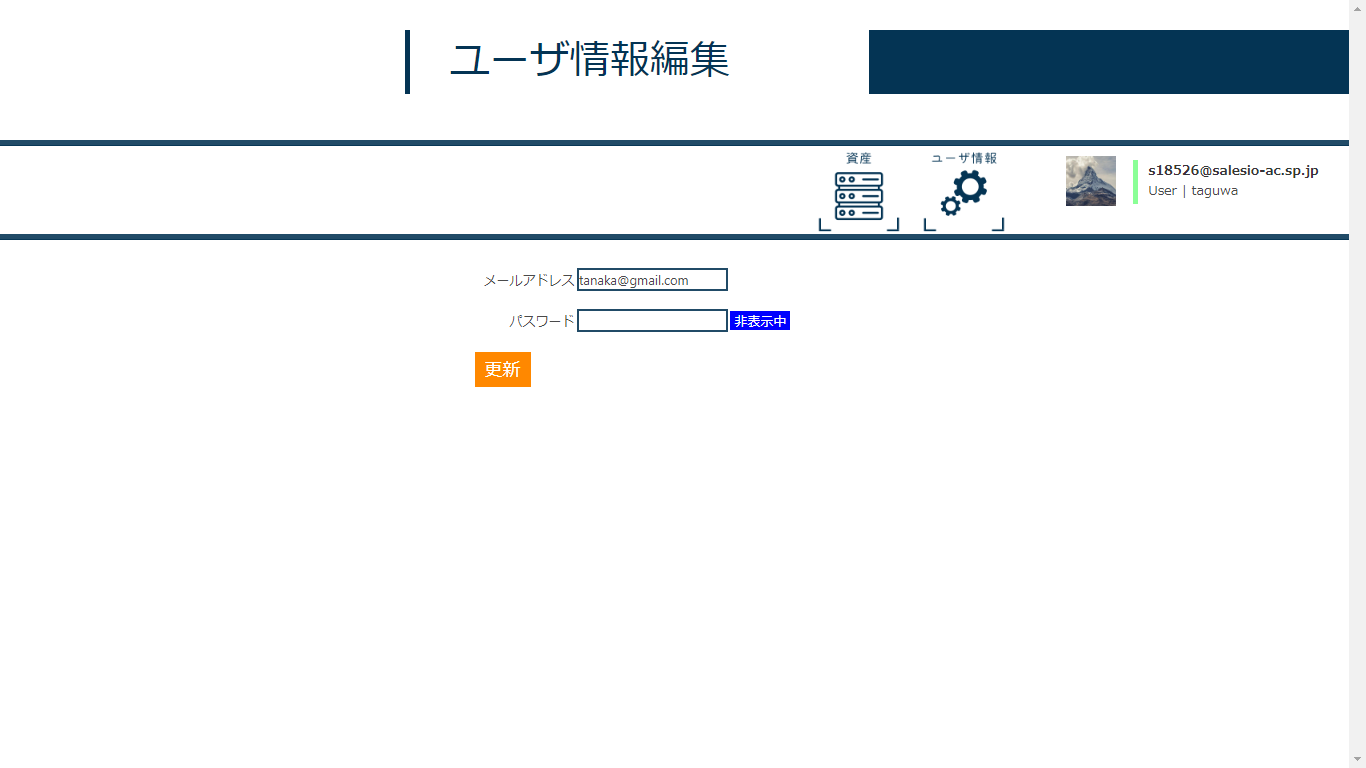
\includegraphics[keepaspectratio, width=0.8\linewidth]{source/user_edit.png}
%   }
%   \caption{\label{fig:プロフィールの編集画面}プロフィールの編集画面}
% \end{figure}


% \section{プロフィールの編集}なので、コメントアウトしました 2023/01/13 11:59 高橋


%%%%%%%%%%
\clearpage
\section{ユーザの管理}
\label{sec:ユーザの管理}
本システムに登録されているユーザを一覧し、管理することができます。一覧は学科ごとに分かれて表示され、各データには\ovalbox{削除}ボタンが付属しています。\ovalbox{削除}ボタンを押すと確認画面(図\ref{fig:ユーザの管理画面の確認表示})が表示され、\ovalbox{{\sf OK}}ボタンを押すと登録できます
%・ユーザ管理
\begin{figure}[h]
  \centering
  \fbox{
    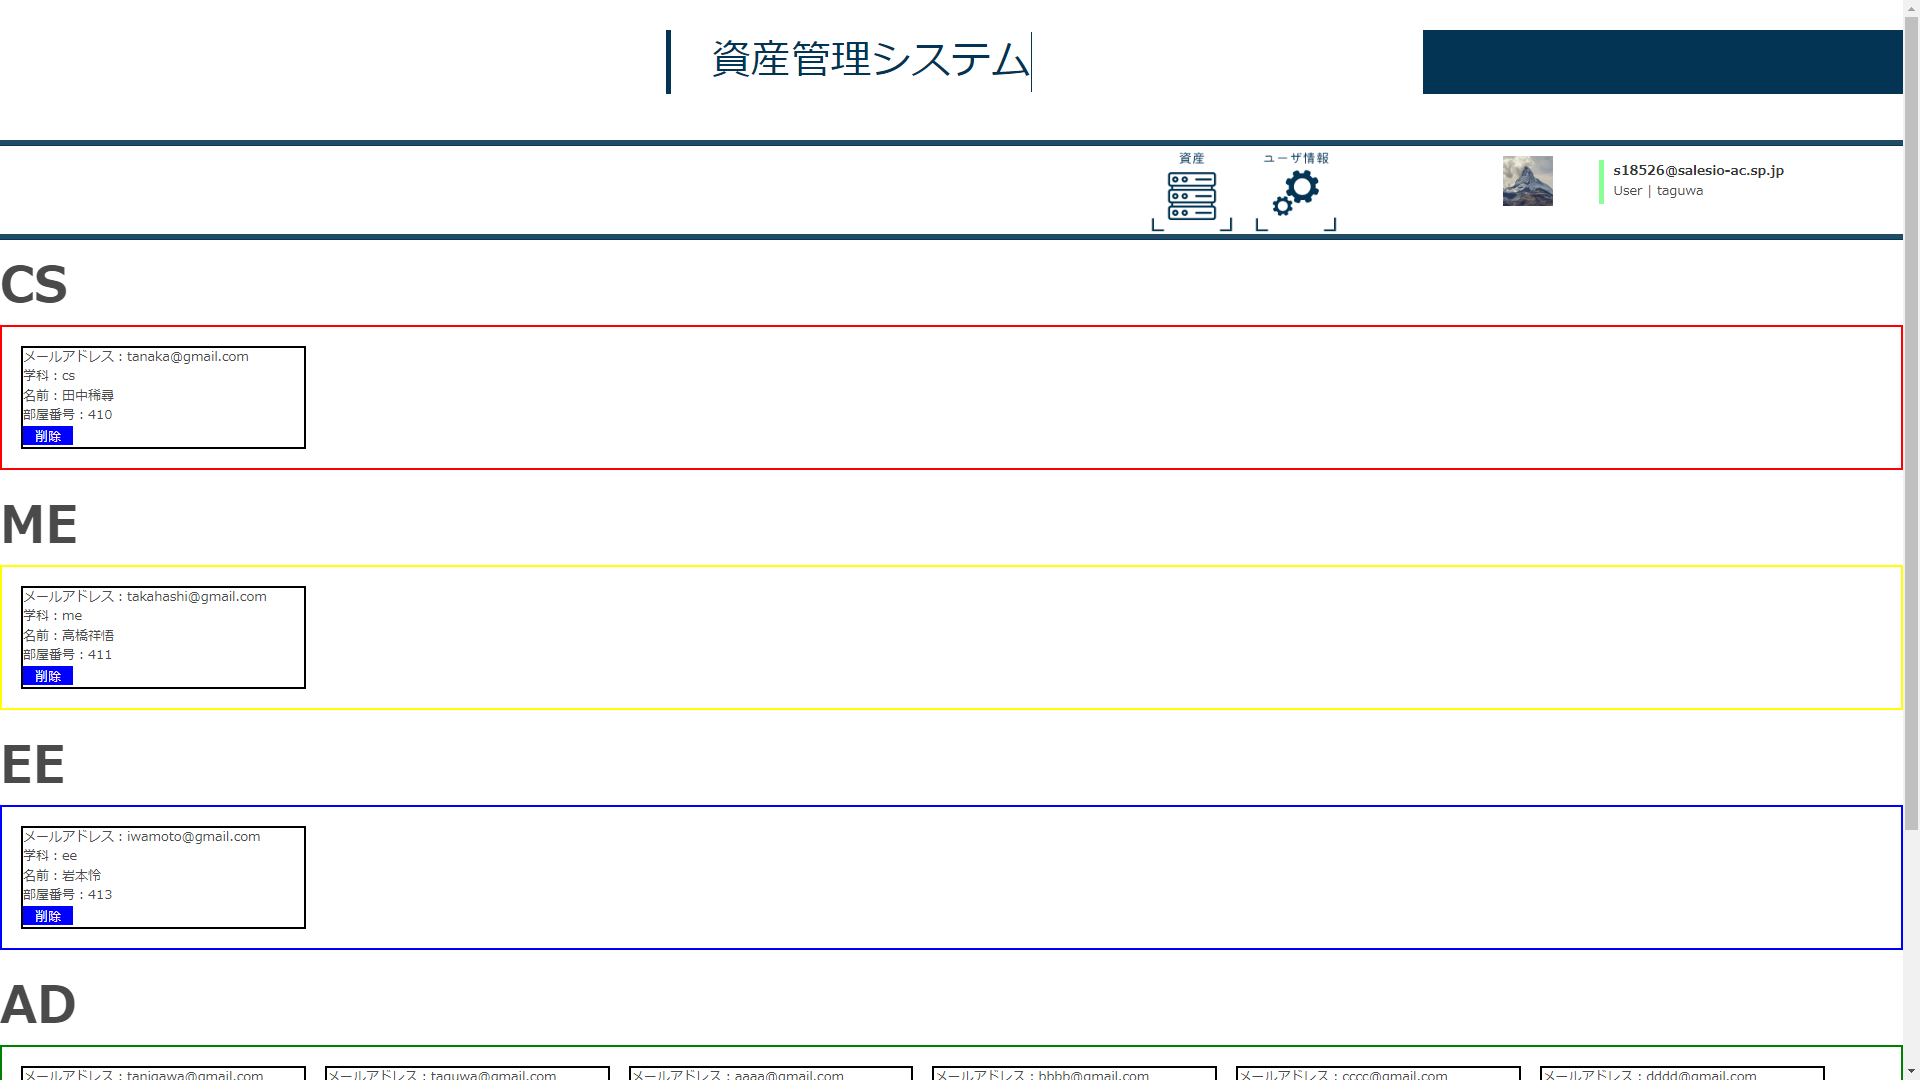
\includegraphics[keepaspectratio, width=0.8\linewidth]{source/user_administration.png}
  }
  \caption{\label{fig:ユーザの管理画面}ユーザの管理画面}
\end{figure}
\begin{figure}[h]
  \centering
  \fbox{
    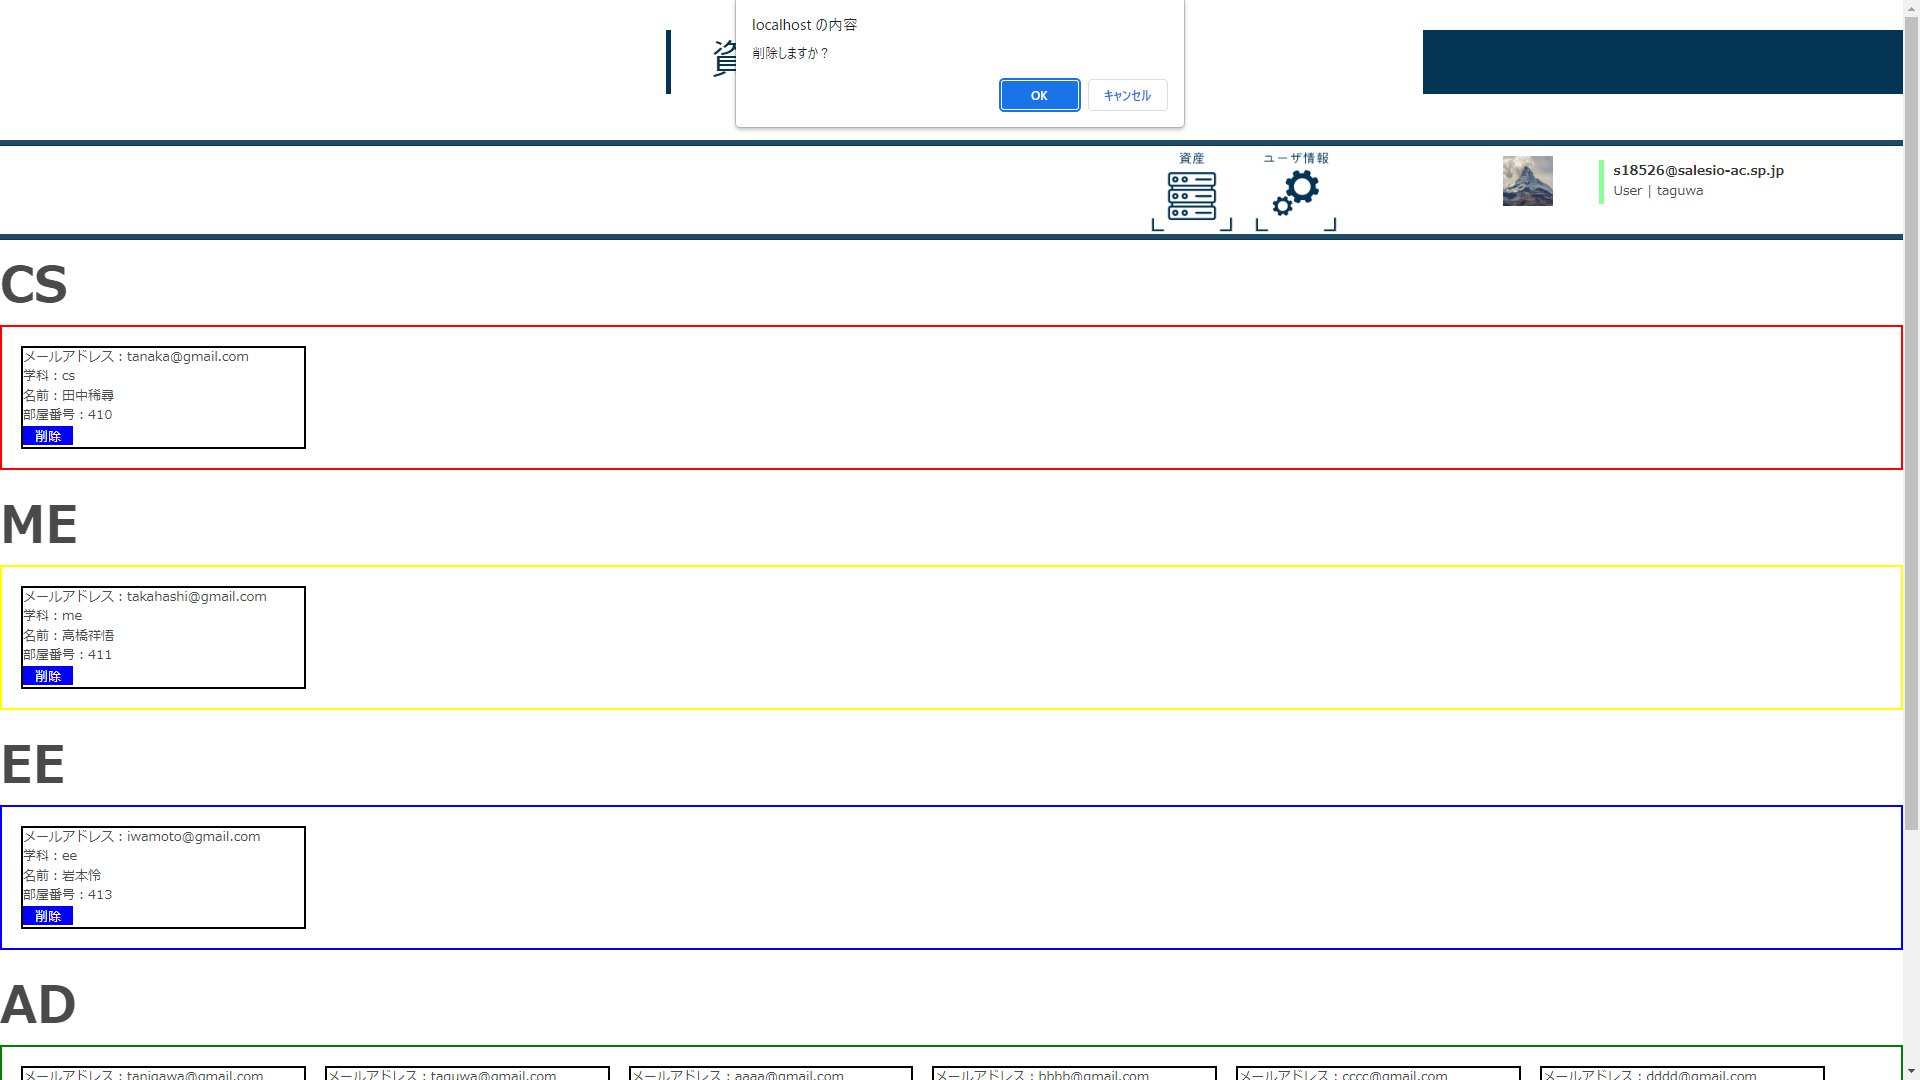
\includegraphics[keepaspectratio, width=0.8\linewidth]{source/user_administration_verification.png}
  }
  \caption{\label{fig:ユーザの管理画面の確認表示}ユーザの管理画面の確認表示}
\end{figure}


%%%%%%%%%%
\clearpage
\section{管理者のパスワード変更}
\label{sec:管理者のパスワード変更}
%管理者のパスワードを変更することができます。パスワードを変更するとき、変更したときは関係者に通達することを推奨します。
2023/01/15 23:42現在 htmlのファイルだけある


%%%%%%%%%%
\clearpage
\section{ユーザの新規追加}
\label{sec:ユーザの新規追加}
\hspace{-1em}・ユーザの新規追加はadminしか行えない\\
・追加するユーザのデータのうち、パスワードは初期は固定値passwordが与えられる\\
・ユーザを追加するとき、チェックボックスで新規追加するユーザがadminなのかfollowerなのか決める\\
・ユーザの新規追加はadminしか行えないので、始祖のadminはDBに直接書きこまれたものを用いる


%%%%%%%%%%
%改変履歴
\clearpage
{\Large\bfseries\ 改変履歴}
\begin{table}[htbp]
  %\caption{}
  %\label{tb:}
  \centering
  \begin{tabularx}{\textwidth}{wc{0.2\linewidth}|wl{0.6\linewidth}|wl{0.2\linewidth}}
    日付       & 項目       & 担当者 \\
    \hline \hline
    2022/12/02 & 初版作成   & 高橋   \\
    \hline
    2023/01/10 & 全体を編集 & 高橋   \\
    %\hline
  \end{tabularx}
\end{table}


\end{document}
%%%%%%%%%%%%%%%%%%%
%%%%%%%%%%%%%%%%%%%

%
